
\documentclass[10pt,openany,a4paper]{article}
\usepackage{tikz, pgfplots, tkz-euclide,calc}
\usetikzlibrary{patterns,shapes.arrows,calc}
\usepackage{fancyhdr}
\usepackage{enumerate,enumitem}
\usepackage{cancel}
\usepackage{varwidth}

% TAMBAHKAN PACKAGE SENDIRI KALAU KURANG

\usepackage{geometry}
\geometry{
	left = 22mm,
	right = 22mm,
	top = 25mm,
	bottom = 25mm,
}
\usepackage{graphicx}
\usepackage{subcaption}
\usepackage{soul}
\usepackage{hyperref}
\usepackage{float}
\usepackage{setspace}
\usepackage{afterpage}
\usepackage{xcolor}
\usepackage[nosectionbib]{apacite}
\usepackage{lmodern}
\usepackage{mathtools}
\usepackage{upgreek}
\usepackage{siunitx}
% \usepackage{fontawesome5}
\usepackage{fontawesome6}
\usepackage{physics}
\usepackage{pdfpages}
\usepackage{hyperref}
\renewcommand{\baselinestretch}{1.3}
\usepackage{multicol}
\usepackage{hyperref,ragged2e,amsmath,multicol,gensymb,setspace,
fancyhdr,amsfonts,tikz,pgfplots,nccmath,enumerate,verbatim,amsthm,physics}
\usepgfplotslibrary{polar,fillbetween}
% Disable tikz externalization to avoid requiring -shell-escape
\usepgfplotslibrary{external}
\tikzexternalize[prefix=tikz/]
\tikzset{reuse path/.code={\pgfsyssoftpath@setcurrentpath{#1}}}
\usetikzlibrary{shapes.geometric,arrows}
\newcommand\mylog[1]{\mathop{{}^{#1}\mathrm{log}}}
\pgfplotsset{compat=1.15}
\pgfplotsset{my style/.append style={axis x line=middle, axis y line=
middle, xlabel={$x$}, ylabel={$y$}, axis equal }}
\usepackage{etoolbox}
% remove stray \makeatother
\newtheorem{defn}{Definisi}[section]
\newtheorem{teo}[defn]{Teorema}
\newtheorem{thm}{Teorema}[section]
\newtheorem{lemma}{Lemma}
\newtheorem{lemmas}[defn]{Lemma}
\newtheorem{cor}[defn]{Akibat}
\newtheorem{asumsi}[defn]{Asumsi}
\theoremstyle{definition}
\newtheorem{con}{Contoh}[section]
\theoremstyle{definition}
\theoremstyle{plain}
\newtheorem{prop}{Proposisi}[section]
\renewcommand{\proofname}{Bukti}
\renewcommand{\thethm}{\arabic{chapter}.\arabic{thm}}

\newcommand{\normlp}[1]{\left\|#1\right\|_{L^p_{\lambda}(0,T;H)}}% Fungsi norm (||x||)
\newcommand{\R}{\mathbb{R}}
\renewcommand{\natural}{\mathbb{N}}
\newcommand{\Xpl}{X^R_{p,\lambda}}
\newcommand{\Xpls}{X^R_{p,\lambda^*}}
\newcommand{\qpl}{q^R_{p,\lambda}}
\newcommand{\qpls}{q^R_{p,\lambda^*}}
\pagestyle{fancy}
\fancyhf{}
\lhead{Halaman \thepage}
% \cfoot{\faXTwitter\ \href{https://x.com/ahmadzakiyudin_/}{@ahmadzakiyudin\_} | \faInstagram\ \href{https://instagram.com/ahmadzakiyudin_/}{@ahmadzakiyudin\_} | \faTiktok\ \href{https://tiktok.com/@ahmathz/}{@ahmathz}}
% \rhead{Pembahasan Soal ETS \\ Kalkulus 1 ITS 2025/2026}
\hypersetup{
    colorlinks=true,
    linkcolor=blue,
    filecolor=blue,      
    urlcolor=blue,
}
\newenvironment{jawab}[2][tes]{
% \fbox{\begin{minipage}{14.65cm}
\textbf{Kata kunci materi:} #1.\\
\textbf{Penyelesaian:} #2
% \end{minipage}}
}{}

\newenvironment{jawab2}[2][tes]{
\fbox{\begin{minipage}{14.65cm}
 #2
\end{minipage}}}{}

\newenvironment{jawaban}[2][tes]{
\colorlet{oldcolor}{.}
        \color{red}
        \setlength{\fboxrule}{1pt}\boxed{\color{oldcolor}#2}\color{oldcolor}.
}{}

\newenvironment{jawaban2}[2][tes]{
\colorlet{oldcolor}{.}
        \color{red}
        \setlength{\fboxrule}{1pt}\fbox{\color{oldcolor}#2}\color{oldcolor}.
}{}

\newenvironment{penting}[2][tes]{
\colorlet{oldcolor}{.}
\color{blue}
\fbox{\color{oldcolor}#2}\color{oldcolor}
}{}

\begin{document}
% \begin{titlepage}
%     \vspace*{\fill}
%     \begin{center}
%       \Huge {PEMBAHASAN SOAL EAS \\ KALKULUS II \\ TAHUN 2024/2025}\\[0.4 cm]
%       \huge {Ahmad Hisbu Zakiyudin}\\[0.2 cm]
%       \Large {(\href{https://instagram.com/ahmadzakiyudin_/}{@ahmadzakiyudin\_})}
%     \end{center}
%     \vspace*{\fill}
%   \end{titlepage}
% !TEX root = ../../BookTemplate.tex
%%%%%%%%%%%%%%%%%%%%%%%%%%%%%%%%%%%%%%%%%%%%%%%%%%%%%%%%%%%%%%%%%%%%%%%%%%%%%%%%%%
% \begin{titlepage}
%     \raggedleft	
% 	\hspace{.025\textwidth}
% 	\parbox[b]{\textwidth}{
%     \vspace{1.5cm}
% 		{\Huge\bfseries Pembahasan Soal EAS}                \\[20pt]
% 		{\huge\textit\ Kalkulus II}\\ \\[10pt]
%         {\Large\textsc{Tahun 2024/2025}}}
% \vfill
% \rule{1pt}{.14\textheight}
% \hspace{.025\textwidth}
%     \raisebox{10pt}{\parbox[b]{.95\textwidth}{ 
%         {\Large\textsc{Ahmad Hisbu Zakiyudin}}              \\[10pt]
%         \large{\href{https://instagram.com/ahmadzakiyudin_/}{@ahmadzakiyudin\_}}               \\[25pt]
%         {\large 5 Juni 2026}}}
% \end{titlepage}
\begin{titlepage}
	\centering % Center everything on the title page
	% \scshape % Use small caps for all text on the title page
	\vspace*{1.5\baselineskip} % White space at the top of the page
% ===================
%	Title Section 	
% ===================

	\rule{13cm}{1.6pt}\vspace*{-\baselineskip}\vspace*{2pt} % Thick horizontal rule
	\rule{13cm}{0.4pt} % Thin horizontal rule
	
		\vspace{0.75\baselineskip} % Whitespace above the title
% ========== Title ===============	
	{	\Huge Soal Tryout ETS\\ 
			\vspace{4mm}
		Kalkulus 1 \\ \vspace{2mm} \huge{Tahun 2026/2027}\\ \vspace{2mm} \Large{(Paket 4)}\\	}
% ======================================
		\vspace{0.75\baselineskip} % Whitespace below the title
	\rule{13cm}{0.4pt}\vspace*{-\baselineskip}\vspace{3.2pt} % Thin horizontal rule
	\rule{13cm}{1.6pt} % Thick horizontal rule
	
		\vspace{1.75\baselineskip} % Whitespace after the title block
% =================
%	Information	
% =================
{\large Oleh: Ahmad Hisbu Zakiyudin}
	% {\large Oleh: Ahmad Hisbu Zakiyudin \\
	% 	\vspace*{1.2\baselineskip}
	% \href{https://instagram.com/ahmadzakiyudin_/}{@ahmadzakiyudin\_}} \\
	\vfill
	\vspace{1mm}
\huge{Selamat Belajar!}
\end{titlepage}
\makeatletter
\setlength\fboxsep{3pt}
% ensure enough header height for fancyhdr
\setlength{\headheight}{24pt}
% Kop tiap kelompok: #1 kelompok, #2 kelas, #3 departemen, #4 jadwal kuliah, #5 sesi
\newcommand{\kopsoal}[5]{%
 \begin{center}
	{\underline{\textbf{\MakeUppercase{Tryout ETS Kalkulus 1 Tahun 2026/2027}}}}
    \end{center}

    \begin{center}
	\begin{tabular}{lcl}
		Mata kuliah/SKS & : & Kalkulus 1 ( SM234101 ) / 3 SKS\\
		Kelompok & : & #1\\
		Kelas & : & #2\\
		Departemen & : & #3\\
		Jadwal kuliah & : & #4\\
		Sesi & : & #5\\
		Waktu & : & 100 menit\\
		Sifat & : & Tertutup\\
  ~
	\end{tabular}

    \noindent\rule{\textwidth}{2.pt}
        \end{center}}

% Kop kelompok IUP (bahasa Inggris): #1 kelompok, #2 kelas, #3 departemen, #4 jadwal kuliah, #5 sesi
\newcommand{\kopsoaliup}[5]{%
 \begin{center}
	{\underline{\textbf{\MakeUppercase{Tryout ETS Kalkulus 1 Tahun 2026/2027}}}}
    \end{center}

    \begin{center}
	\begin{tabular}{lcl}
		Course / Credit & : & Kalkulus 1 ( SM234101 ) / 3 SKS\\
		Group & : & #1\\
		Class & : & #2\\
		Department & : & #3\\
		Lecture schedule & : & #4\\
		Session & : & #5\\
		Time & : & 100 minutes\\
		Type & : & Closed\\
  ~
	\end{tabular}

    \noindent\rule{\textwidth}{2.pt}
        \end{center}}

% Kop tryout Matematika 2 SKS: #1 kelompok, #2 kelas, #3 departemen, #4 jadwal kuliah, #5 sesi
\newcommand{\kopsoalmat}[5]{%
 \begin{center}
	{\underline{\textbf{\MakeUppercase{Tryout ETS Matematika Tahun 2026/2027}}}}
    \end{center}

    \begin{center}
	\begin{tabular}{lcl}
		Mata kuliah/SKS & : & Matematika ( SM234152 ) / 2 SKS\\
		Kelompok & : & #1\\
		Kelas & : & #2\\
		Departemen & : & #3\\
		Jadwal kuliah & : & #4\\
		Sesi & : & #5\\
		Waktu & : & 100 menit\\
		Sifat & : & Tertutup\\
  ~
	\end{tabular}

    \noindent\rule{\textwidth}{2.pt}
        \end{center}}

% Kop tryout Matematika 2 SKS IUP (bahasa Inggris)
\newcommand{\kopsoalmatiup}[5]{%
 \begin{center}
	{\underline{\textbf{\MakeUppercase{Tryout ETS Matematika Tahun 2026/2027}}}}
    \end{center}

    \begin{center}
	\begin{tabular}{lcl}
		Course / Credit & : & Matematika ( SM234152 ) / 2 SKS\\
		Group & : & #1\\
		Class & : & #2\\
		Department & : & #3\\
		Lecture schedule & : & #4\\
		Session & : & #5\\
		Time & : & 100 minutes\\
		Type & : & Closed\\
  ~
	\end{tabular}

    \noindent\rule{\textwidth}{2.pt}
        \end{center}}

%%%%%%%%%%%%%%%%%%%%%%%%%%%%%%%%%%%%%%%%%%%%%%%%%%%%%%%%%%%%%%%%%%%%%%%%%%%%%%
% Kal-5 | Paket 4: subbab per nomor 1.1, 2.3, 2.4, 3.3, 4.2
% Kisi-kisi hari Senin: subbab 1.1, 1.5, 2.3, 2.4, 3.1, 3.3, 4.2, 4.4
\kopsoal{Kal-5}{22-27}{T. Fisika, T. Material dan Metalurgi, Rkp}{Senin, Rabu; 07.00-09.30}{1}
\begin{enumerate}
    \item \textbf{[Subbab 1.1]} Dapatkan himpunan penyelesaian pertidaksamaan
    \begin{align*}
        \frac{x}{x-2}\leq\frac{3}{x+2}.
    \end{align*}

    \item \textbf{[Subbab 2.3]} Diberikan $f(x)=x^2-4|x|$.
    \begin{enumerate}
        \item Nyatakan $f(x)$ sebagai fungsi sepotong-sepotong tanpa tanda mutlak.
        \item Sketsa grafik $f$, kemudian tandai titik-titik potongnya dengan sumbu-$x$ dan titik-titik terendahnya.
    \end{enumerate}

    \item \textbf{[Subbab 2.4]} Diberikan fungsi $f(x)=\dfrac{2-x}{x+3}$.
    \begin{enumerate}
        \item Tentukan domain dan range dari $f$.
        \item Dapatkan $f^{-1}(x)$ beserta domainnya.
    \end{enumerate}

    \item \textbf{[Subbab 3.3]} Hitunglah $\displaystyle\lim_{x\to+\infty}\left(\sqrt{x^2+x+1}-\sqrt{x^2-x}\right)$.

    \item \textbf{[Subbab 4.2]} Selidiki apakah fungsi
    \begin{align*}
        f(x)=\begin{cases}
            x^3, & x\leq 1\\
            3x-2, & x>1
        \end{cases}
    \end{align*}
    dapat diturunkan di $x=1$. Jika dapat, tentukan $f'(1)$.
\end{enumerate}

\newpage

%%%%%%%%%%%%%%%%%%%%%%%%%%%%%%%%%%%%%%%%%%%%%%%%%%%%%%%%%%%%%%%%%%%%%%%%%%%%%%
% Kal-6 | Paket 4: subbab per nomor 1.1, 2.3, 2.4, 3.3, 4.2
% Kisi-kisi hari Senin: subbab 1.1, 1.5, 2.3, 2.4, 3.1, 3.3, 4.2, 4.4
\kopsoal{Kal-6}{28-31}{T. Perkapalan, T. Transportasi Laut, T. Bangunan Lepas Pantai}{Senin, Rabu; 07.00-09.30}{1}
\begin{enumerate}
    \item \textbf{[Subbab 1.1]} Selesaikan pertidaksamaan berikut
    \begin{align*}
        -2<x^2-3x\leq 4.
    \end{align*}

    \item \textbf{[Subbab 2.3]} Grafik fungsi $y=f(x)$ dengan domain $[-4,4]$ terdiri dari dua ruas garis seperti pada gambar berikut.
    \begin{center}
        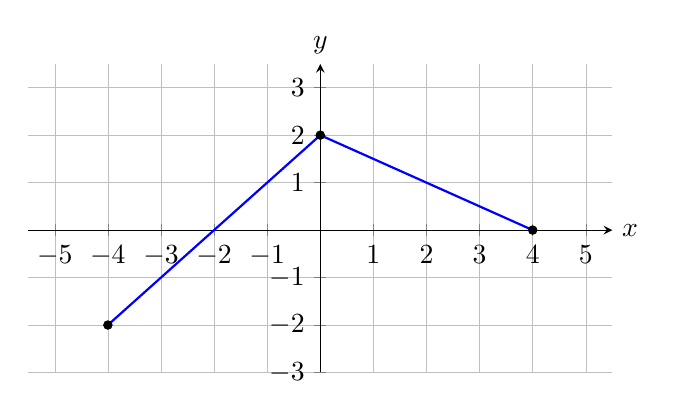
\begin{tikzpicture}
            \begin{axis}[
        axis lines = middle,
        xlabel = $x$,
        ylabel = {$y$},
        grid=both,
        grid style={line width=.1pt, draw=gray!10},
        major grid style={line width=.2pt,draw=gray!50},
        x label style={anchor=west}, % label x ke kanan
        y label style={anchor=south}, % label y ke atas
        samples=200,
        legend style={
                at={(1.1,1)},
                anchor=north west,
                font=\small,         % mengecilkan ukuran font
                row sep=1pt,         % jarak antar baris legend
                inner sep=1pt,       % margin dalam kotak legend
                nodes={scale=0.7}    % skalakan isi legend
            },
        xtick={-5,-4,...,5},
        ytick={-3,-2,...,3},
        xmin=-5.5, xmax=5.5,
        ymin=-3, ymax=3.5,
        width=9cm,
        height=5.5cm
    ]
\addplot[color=blue, thick] coordinates {(-4,-2) (0,2) (4,0)};
\draw[fill=black] (-4,-2) circle (1.5pt);
\draw[fill=black] (0,2) circle (1.5pt);
\draw[fill=black] (4,0) circle (1.5pt);
\end{axis}
        \end{tikzpicture}
    \end{center}
    \begin{enumerate}
        \item Tentukan rumus $f(x)$ sebagai fungsi sepotong-sepotong.
        \item Tentukan semua $x$ yang memenuhi $f(x)=1$.
        \item Tentukan semua $x$ yang memenuhi $f(x)\geq 0$.
    \end{enumerate}

    \item \textbf{[Subbab 2.4]} Diberikan fungsi $f(x)=\sqrt{x^2-4}$ dengan $x\geq 2$.
    \begin{enumerate}
        \item Tentukan range dari $f$.
        \item Dapatkan $f^{-1}(x)$ beserta domainnya.
    \end{enumerate}

    \item \textbf{[Subbab 3.3]} Hitunglah $\displaystyle\lim_{x\to-\infty}\frac{\sqrt{4x^2+1}}{x-1}$.

    \item \textbf{[Subbab 4.2]} Dengan menggunakan definisi turunan, dapatkan $f'(x)$ dari $f(x)=x^2-5x$. Kemudian tentukan kemiringan garis singgung kurva $y=f(x)$ di $x=2$.
\end{enumerate}

\newpage

%%%%%%%%%%%%%%%%%%%%%%%%%%%%%%%%%%%%%%%%%%%%%%%%%%%%%%%%%%%%%%%%%%%%%%%%%%%%%%
% Kal-iup-1 | Paket 4: subbab per nomor 1.1, 2.3, 2.4, 3.1, 4.2
% Kisi-kisi hari Senin: subbab 1.1, 1.5, 2.3, 2.4, 3.1, 3.3, 4.2, 4.4
\kopsoaliup{Kal-iup-1}{61, 68}{Chemical, Environmental, Electrical Engineering}{Monday, Wednesday; 07.00-09.30}{1}
\begin{enumerate}
    \item \textbf{[Subbab 1.1]} Solve the following inequality.
    \begin{align*}
        \frac{x^2-x-2}{x^2+x+2}\geq 0.
    \end{align*}

    \item \textbf{[Subbab 2.3]} Sketch the graph of $f(x)=\sqrt{x+2}$ and the line $y=x$ on the same coordinate plane. Then, find the intersection point of the two graphs.

    \item \textbf{[Subbab 2.4]} Given a function $f(x)=x^2+4x+1$ with $x\geq -2$. Determine:
    \begin{enumerate}
        \item[a)] The range of $f$;
        \item[b)] $f^{-1}(x)$ and its domain;
        \item[c)] Sketch the graph of $f(x)$ and $f^{-1}(x)$ in the same coordinate plane.
    \end{enumerate}

    \item \textbf{[Subbab 3.1]} Sketch the graph of a function $f$ that satisfies all of the following conditions (many answers are possible):
    \begin{enumerate}
        \item[a.] the domain of $f$ is $[-1,+\infty)$,
        \item[b.] $f(-1)=f(3)=0$,
        \item[c.] $\displaystyle\lim_{x\to 1^-}f(x)=4$, $\displaystyle\lim_{x\to 1^+}f(x)=2$, $\displaystyle\lim_{x\to 5}f(x)=1$, but $f(5)=3$.
    \end{enumerate}

    \item \textbf{[Subbab 4.2]} Using the definition of derivative, find $f'(x)$ of $f(x)=x^2+2x-1$. Then, find the equation of the tangent line to the curve $y=f(x)$ at $x=1$.
\end{enumerate}

\newpage

%%%%%%%%%%%%%%%%%%%%%%%%%%%%%%%%%%%%%%%%%%%%%%%%%%%%%%%%%%%%%%%%%%%%%%%%%%%%%%
% Kal-iup-4 | Paket 4: subbab per nomor 1.1, 2.3, 2.4, 3.1, 4.2
% Kisi-kisi hari Senin: subbab 1.1, 1.5, 2.3, 2.4, 3.1, 3.3, 4.2, 4.4
\kopsoaliup{Kal-iup-4}{65, 66, 67}{Statistics, Marine Engineering (JD), Informatics}{Monday, Wednesday; 07.00-09.30}{1}
\begin{enumerate}
    \item \textbf{[Subbab 1.1]} Solve the following inequality.
    \begin{align*}
        \frac{1}{x-1}\leq\frac{2}{x+2}.
    \end{align*}

    \item \textbf{[Subbab 2.3]} Sketch the base curve $y=\sqrt{x}$. Based on that base curve, use reflection and translation to sketch the curve $y=2-\sqrt{x+1}$. (Explain the process).

    \item \textbf{[Subbab 2.4]} Given a function $f(x)=4-(x+1)^3$.
    \begin{enumerate}
        \item[a)] Find $f^{-1}(x)$ and its domain.
        \item[b)] Sketch the graph of $f(x)$ and $f^{-1}(x)$ in the same coordinate plane.
    \end{enumerate}

    \item \textbf{[Subbab 3.1]} Given $f(x)=\sqrt{4-x}+1$.
    \begin{enumerate}
        \item[a.] Determine the domain of $f$ and sketch its graph.
        \item[b.] Find $\displaystyle\lim_{x\to 4^-}f(x)$ and explain why $\displaystyle\lim_{x\to 4^+}f(x)$ does not exist.
    \end{enumerate}

    \item \textbf{[Subbab 4.2]} Find the values of $a$ and $b$ such that the function
    \begin{align*}
        f(x)=\begin{cases}
            ax+b, & x<2\\
            x^2-2x+3, & x\geq 2
        \end{cases}
    \end{align*}
    is continuous and differentiable at $x=2$.
\end{enumerate}

\newpage

%%%%%%%%%%%%%%%%%%%%%%%%%%%%%%%%%%%%%%%%%%%%%%%%%%%%%%%%%%%%%%%%%%%%%%%%%%%%%%
% Kal-9 | Paket 4: subbab per nomor 1.1, 2.3, 2.4, 3.1, 4.2
% Kisi-kisi hari Senin: subbab 1.1, 1.5, 2.3, 2.4, 3.1, 3.3, 4.2, 4.4
\kopsoal{Kal-9}{44-48}{T. Sistem Perkapalan, T. Kelautan, T. Komputer}{Senin, Rabu; 12.30-15.00}{3}
\begin{enumerate}
    \item \textbf{[Subbab 1.1]} Dapatkan himpunan penyelesaian dari
    \begin{align*}
        \frac{(x+2)(x-1)}{(x-3)^2}\geq 0.
    \end{align*}

    \item \textbf{[Subbab 2.3]} Diberikan $f(x)=\begin{cases}
        x+2, & x<0\\
        (x-1)^2+1, & x\geq 0
    \end{cases}$.\\
    Gambarkan sketsa grafik $f$, kemudian tentukan range dari $f$ berdasarkan grafik tersebut.

    \item \textbf{[Subbab 2.4]} Diberikan fungsi $f(x)=\dfrac{1}{x^2+1}$ dengan $x\geq 0$.
    \begin{enumerate}
        \item Tentukan range dari $f$.
        \item Dapatkan $f^{-1}(x)$ beserta domainnya.
    \end{enumerate}

    \item \textbf{[Subbab 3.1]} Tentukan semua nilai $a$ agar $\displaystyle\lim_{x\to 2}f(x)$ ada, dimana
    \begin{align*}
        f(x)=\begin{cases}
            a^2x-2a, & x<2\\
            x+2, & x>2
        \end{cases}.
    \end{align*}

    \item \textbf{[Subbab 4.2]} Diberikan $f(x)=\left|x^2-1\right|$. Selidiki apakah $f$ dapat diturunkan di $x=1$.
\end{enumerate}

\newpage

%%%%%%%%%%%%%%%%%%%%%%%%%%%%%%%%%%%%%%%%%%%%%%%%%%%%%%%%%%%%%%%%%%%%%%%%%%%%%%
% Kal-11 | Paket 4: subbab per nomor 1.1, 2.3, 2.4, 3.3, 4.2
% Kisi-kisi hari Senin: subbab 1.1, 1.5, 2.3, 2.4, 3.1, 3.3, 4.2, 4.4
\kopsoal{Kal-11}{51-54}{Biologi, Bioteknologi, Teknologi Informasi}{Senin, Rabu; 12.30-15.00}{3}
\begin{enumerate}
    \item \textbf{[Subbab 1.1]} Tentukan semua nilai $x$ yang memenuhi pertidaksamaan
    \begin{align*}
        x^3-x^2-6x<0.
    \end{align*}

    \item \textbf{[Subbab 2.3]} Diberikan $f(x)=\left|x^2-2x\right|$.
    \begin{enumerate}
        \item Nyatakan $f(x)$ sebagai fungsi sepotong-sepotong tanpa tanda mutlak.
        \item Sketsa grafik $f$, kemudian tentukan range-nya.
    \end{enumerate}

    \item \textbf{[Subbab 2.4]} Diberikan suatu fungsi $f(x)=3-\sqrt{16-x^2}$ dengan domain $[0,4]$.
    \begin{enumerate}
        \item Tentukan range dari $f$.
        \item Dapatkan $f^{-1}(x)$ beserta domainnya.
        \item Sketsa grafik $f(x)$ dan $f^{-1}(x)$ pada satu bidang koordinat.
    \end{enumerate}

    \item \textbf{[Subbab 3.3]} Hitunglah $\displaystyle\lim_{x\to-\infty}\frac{3x^3-x}{\sqrt{x^6+2x}}$.

    \item \textbf{[Subbab 4.2]} Diketahui
    \begin{align*}
        \lim_{h\to 0}\frac{(3+h)^2-9}{h}
    \end{align*}
    menyatakan turunan suatu fungsi $f$ di suatu titik $x=a$. Tentukan $f$ dan $a$, kemudian hitung nilai limit tersebut.
\end{enumerate}

\newpage

%%%%%%%%%%%%%%%%%%%%%%%%%%%%%%%%%%%%%%%%%%%%%%%%%%%%%%%%%%%%%%%%%%%%%%%%%%%%%%
% Kal-12 | Paket 4: subbab per nomor 1.1, 2.3, 2.4, 3.1, 4.2
% Kisi-kisi hari Senin: subbab 1.1, 1.5, 2.3, 2.4, 3.1, 3.3, 4.2, 4.4
\kopsoal{Kal-12}{55-60}{Aktuaria, Teknik Informatika, RPL, RKA}{Senin, Rabu; 12.30-15.00}{3}
\begin{enumerate}
    \item \textbf{[Subbab 1.1]} Tentukan penyelesaian dari pertidaksamaan
    \begin{align*}
        \frac{x^2+3}{x-1}\geq x+3.
    \end{align*}

    \item \textbf{[Subbab 2.3]} Grafik berikut diperoleh dari kurva dasar $y=\sqrt{x}$ dengan menggunakan translasi.
    \begin{center}
        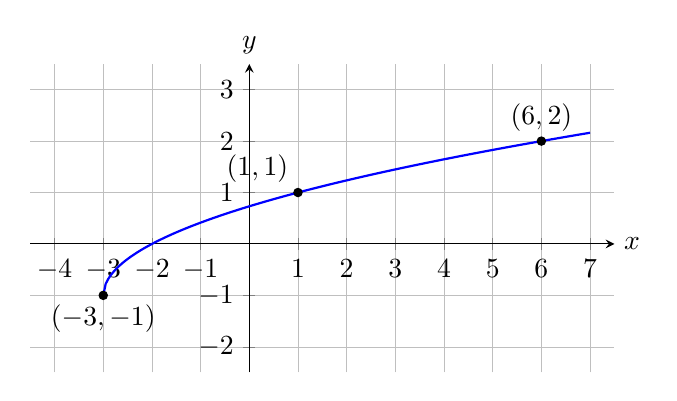
\begin{tikzpicture}
            \begin{axis}[
        axis lines = middle,
        xlabel = $x$,
        ylabel = {$y$},
        grid=both,
        grid style={line width=.1pt, draw=gray!10},
        major grid style={line width=.2pt,draw=gray!50},
        x label style={anchor=west}, % label x ke kanan
        y label style={anchor=south}, % label y ke atas
        samples=200,
        legend style={
                at={(1.1,1)},
                anchor=north west,
                font=\small,         % mengecilkan ukuran font
                row sep=1pt,         % jarak antar baris legend
                inner sep=1pt,       % margin dalam kotak legend
                nodes={scale=0.7}    % skalakan isi legend
            },
        xtick={-4,-3,...,7},
        ytick={-2,-1,...,3},
        xmin=-4.5, xmax=7.5,
        ymin=-2.5, ymax=3.5,
        width=9cm,
        height=5.5cm
    ]
\addplot[domain=-3:7, color=blue, thick] {sqrt(x+3)-1};
\draw[fill=black] (-3,-1) circle (1.5pt) node[below] {$(-3,-1)$};
\draw[fill=black] (1,1) circle (1.5pt) node[above left] {$(1,1)$};
\draw[fill=black] (6,2) circle (1.5pt) node[above] {$(6,2)$};
\end{axis}
        \end{tikzpicture}
    \end{center}
    \begin{enumerate}
        \item Jelaskan translasi yang dilakukan dan tentukan persamaan kurva tersebut.
        \item Tentukan domain, range, dan titik potong kurva dengan sumbu-$x$.
    \end{enumerate}

    \item \textbf{[Subbab 2.4]} Diberikan $f(x)=2x^3-1$.
    \begin{enumerate}
        \item Dapatkan $f^{-1}(x)$ beserta domainnya.
        \item Hitunglah $f^{-1}(15)$, kemudian periksa jawabanmu dengan menghitung $f\big(f^{-1}(15)\big)$.
    \end{enumerate}

    \item \textbf{[Subbab 3.1]} Diberikan $f(x)=\dfrac{x+2}{x(x-1)}$. Dapatkan $\displaystyle\lim_{x\to 0^-}f(x)$, $\displaystyle\lim_{x\to 0^+}f(x)$, $\displaystyle\lim_{x\to 1^-}f(x)$, dan $\displaystyle\lim_{x\to 1^+}f(x)$.

    \item \textbf{[Subbab 4.2]} Dengan menggunakan definisi turunan, dapatkan $f'(1)$ jika $f(x)=x^3-x$. Kemudian dapatkan persamaan garis singgung kurva $y=f(x)$ di $x=1$.
\end{enumerate}

\newpage

%%%%%%%%%%%%%%%%%%%%%%%%%%%%%%%%%%%%%%%%%%%%%%%%%%%%%%%%%%%%%%%%%%%%%%%%%%%%%%
% Kal-7 | Paket 4: subbab per nomor 1.1, 2.3, 2.4, 3.1, 4.2
% Kisi-kisi hari Senin: subbab 1.1, 1.5, 2.3, 2.4, 3.1, 3.3, 4.2, 4.4
\kopsoal{Kal-7}{32-37}{T. Sipil, T. Geomatika, T. Geofisika, T. Pertambangan}{Senin, Rabu; 15.30-17.10}{4}
\begin{enumerate}
    \item \textbf{[Subbab 1.1]} Dapatkan himpunan penyelesaian pertidaksamaan
    \begin{align*}
        \frac{4}{x+1}\geq x-2.
    \end{align*}

    \item \textbf{[Subbab 2.3]} Gunakan kurva dasar $y=\sqrt[3]{x}$ dan sifat pencerminan serta translasi untuk menggambar sketsa grafik $F(x)=2-\sqrt[3]{x+1}$. (Jelaskan prosesnya.)

    \item \textbf{[Subbab 2.4]} Diberikan fungsi $f(x)=\sqrt{x+5}-2$.
    \begin{enumerate}
        \item Tentukan domain dan range dari $f$.
        \item Dapatkan $f^{-1}(x)$ beserta domainnya.
        \item Sketsa grafik $f(x)$ dan $f^{-1}(x)$ pada satu bidang koordinat.
    \end{enumerate}

    \item \textbf{[Subbab 3.1]} Buatlah sketsa grafik suatu fungsi $f$ yang memenuhi semua syarat berikut (banyak jawaban yang mungkin):
    \begin{enumerate}
        \item domain $f$ adalah $[-2,2]$,
        \item $f(-2)=f(0)=f(2)=1$,
        \item $\displaystyle\lim_{x\to -2^+}f(x)=\lim_{x\to 2^-}f(x)=-1$ dan $\displaystyle\lim_{x\to 0}f(x)=3$.
    \end{enumerate}

    \item \textbf{[Subbab 4.2]} Dengan menggunakan definisi turunan, dapatkan turunan dari $f(x)=\dfrac{1}{x}$. Kemudian dapatkan semua titik pada kurva $y=\dfrac{1}{x}$ yang garis singgungnya bergradien $-\frac{1}{4}$, beserta persamaan garis singgungnya.
\end{enumerate}

\newpage

%%%%%%%%%%%%%%%%%%%%%%%%%%%%%%%%%%%%%%%%%%%%%%%%%%%%%%%%%%%%%%%%%%%%%%%%%%%%%%
% Kal-8 | Paket 4: subbab per nomor 1.1, 1.5, 2.4, 3.1, 4.2
% Kisi-kisi hari Senin: subbab 1.1, 1.5, 2.3, 2.4, 3.1, 3.3, 4.2, 4.4
\kopsoal{Kal-8}{38-43}{Matematika, Statistika, Sains Data}{Senin, Rabu; 15.30-17.10}{4}
\begin{enumerate}
    \item \textbf{[Subbab 1.1]} Dapatkan himpunan penyelesaian pertidaksamaan
    \begin{align*}
        \frac{x^2-4x}{x^2-4x+3}\geq 0.
    \end{align*}

    \item \textbf{[Subbab 1.5]} Sebuah batu dilempar lurus ke atas sehingga setelah $t$ detik ketinggiannya dari titik pelemparan adalah $s=40t-8t^2$ meter.
    \begin{enumerate}
        \item Gambarkan grafik persamaan tersebut pada bidang koordinat-$ts$ (sumbu-$t$ horisontal).
        \item Pada waktu $t$ berapakah batu mencapai titik tertingginya, dan berapa ketinggian titik tersebut?
        \item Kapan batu kembali ke titik pelemparan?
    \end{enumerate}

    \item \textbf{[Subbab 2.4]} Diberikan fungsi $f(x)=2-(x-1)^2$ dengan $x\geq 1$.
    \begin{enumerate}
        \item Tentukan range dari $f$.
        \item Dapatkan $f^{-1}(x)$ beserta domainnya.
        \item Sketsa grafik $f(x)$ dan $f^{-1}(x)$ pada satu bidang koordinat.
    \end{enumerate}

    \item \textbf{[Subbab 3.1]} Diberikan $f(x)=\begin{cases}
        2-x, & x\leq 1\\
        x^2+1, & x>1
    \end{cases}$.
    \begin{enumerate}
        \item Sketsa grafik $f$.
        \item Selidiki apakah $\displaystyle\lim_{x\to 1}f(x)$ dan $\displaystyle\lim_{x\to 2}f(x)$ ada.
    \end{enumerate}

    \item \textbf{[Subbab 4.2]} Garis singgung kurva $y=f(x)$ di titik dengan absis $x=2$ adalah $y=3x-4$.
    \begin{enumerate}
        \item Tentukan $f(2)$ dan $f'(2)$.
        \item Jika $f(x)=x^2+ax+b$, gunakan definisi turunan untuk mendapatkan $f'(x)$, kemudian tentukan nilai $a$ dan $b$.
    \end{enumerate}
\end{enumerate}

\newpage

%%%%%%%%%%%%%%%%%%%%%%%%%%%%%%%%%%%%%%%%%%%%%%%%%%%%%%%%%%%%%%%%%%%%%%%%%%%%%%
% Kal-iup-2 | Paket 4: subbab per nomor 1.1, 2.3, 2.4, 3.1, 4.2
% Kisi-kisi hari Senin: subbab 1.1, 1.5, 2.3, 2.4, 3.1, 3.3, 4.2, 4.4
\kopsoaliup{Kal-iup-2}{62, 69}{Mechanical, Industrial, Materials \& Metallurgical Engineering}{Monday, Wednesday; 15.30-17.10}{4}
\begin{enumerate}
    \item \textbf{[Subbab 1.1]} Find the solution of the following inequality
    \begin{align*}
        \frac{x+1}{x-2}\geq -1.
    \end{align*}

    \item \textbf{[Subbab 2.3]} Sketch the base curve $y=x^2$. Based on that base curve, use reflection and translation to sketch the curve $y=4-(x-1)^2$, and determine its vertex and its intersection points with the coordinate axes. (Explain the process).

    \item \textbf{[Subbab 2.4]} Given a function $f(x)=\dfrac{4x-1}{x+2}$. Determine:
    \begin{enumerate}
        \item[a)] The domain and range of $f$;
        \item[b)] $f^{-1}(x)$ and its domain.
    \end{enumerate}

    \item \textbf{[Subbab 3.1]} Given $f(x)=\dfrac{x-2}{x^2-4}$.
    \begin{enumerate}
        \item[a.] Find $\displaystyle\lim_{x\to 2}f(x)$.
        \item[b.] Find $\displaystyle\lim_{x\to -2^-}f(x)$ and $\displaystyle\lim_{x\to -2^+}f(x)$.
    \end{enumerate}

    \item \textbf{[Subbab 4.2]} Show that $f(x)=\begin{cases}
        x^2, & x\leq 1\\
        2x-1, & x>1
    \end{cases}$ is continuous and differentiable at $x=1$.
\end{enumerate}

\newpage

%%%%%%%%%%%%%%%%%%%%%%%%%%%%%%%%%%%%%%%%%%%%%%%%%%%%%%%%%%%%%%%%%%%%%%%%%%%%%%
% Kal-3 | Paket 4: subbab per nomor 1.2, 1.4, 2.1, 3.4, 4.2
% Kisi-kisi hari Selasa: subbab 1.2, 1.4, 2.1, 2.2, 3.2, 3.4, 4.2, 4.3
\kopsoal{Kal-3}{13-16}{Kimia, Saik, Telkom}{Selasa, Kamis; 07.00-09.30}{6}
\begin{enumerate}
    \item \textbf{[Subbab 1.2]} Tentukan himpunan penyelesaian dari
    \begin{align*}
        \left|x^2-5x\right|=6.
    \end{align*}

    \item \textbf{[Subbab 1.4]} Diberikan titik $A(0,4)$, $B(4,0)$, dan $C(5,5)$. Misalkan $M$ adalah titik tengah ruas garis $AB$.
    \begin{enumerate}
        \item Tentukan koordinat $M$ dan panjang ruas garis $CM$.
        \item Dapatkan persamaan garis yang melalui titik $(3,-2)$ dan sejajar dengan garis $CM$.
    \end{enumerate}

    \item \textbf{[Subbab 2.1]} Tentukan domain dan range dari fungsi $f(x)=\sqrt{\dfrac{x^2-9}{x-3}}$.

    \item \textbf{[Subbab 3.4]} Dapatkan nilai $k$ sedemikian sehingga fungsi
    \begin{align*}
        f(x)=\begin{cases}
            kx+1, & x<2\\
            x^2-k, & x\geq 2
        \end{cases}
    \end{align*}
    kontinu di $x=2$.

    \item \textbf{[Subbab 4.2]} Dengan menggunakan definisi turunan, dapatkan $f'(x)$ dari $f(x)=x^2+4x$. Kemudian tentukan titik pada kurva $y=f(x)$ yang garis singgungnya mendatar.
\end{enumerate}

\newpage

%%%%%%%%%%%%%%%%%%%%%%%%%%%%%%%%%%%%%%%%%%%%%%%%%%%%%%%%%%%%%%%%%%%%%%%%%%%%%%
% Kal-4 | Paket 4: subbab per nomor 1.2, 1.4, 2.2, 3.2, 4.2
% Kisi-kisi hari Selasa: subbab 1.2, 1.4, 2.1, 2.2, 3.2, 3.4, 4.2, 4.3
\kopsoal{Kal-4}{17-21}{T. Mesin, Teknik Sistem dan Industri}{Selasa, Kamis; 07.00-09.30}{6}
\begin{enumerate}
    \item \textbf{[Subbab 1.2]}
    \begin{enumerate}
        \item Nyatakan $\sqrt{x^2+6x+9}$ dalam bentuk nilai mutlak.
        \item Dapatkan semua nilai $x$ yang memenuhi persamaan $\sqrt{x^2+6x+9}=2x-3$.
    \end{enumerate}

    \item \textbf{[Subbab 1.4]}
    \begin{enumerate}
        \item Gunakan gradien untuk menentukan apakah titik-titik $(2,1)$, $(4,4)$, dan $(-2,-5)$ terletak pada satu garis lurus.
        \item Tentukan nilai $k$ agar titik-titik $(k,2)$, $(1,-1)$, dan $(3,5)$ terletak pada satu garis lurus, kemudian tentukan persamaan garis tersebut.
    \end{enumerate}

    \item \textbf{[Subbab 2.2]} Diberikan $f(x)=\dfrac{x}{x+2}$ dan $g(x)=\dfrac{2}{x-1}$.
    \begin{enumerate}
        \item Dapatkan $(f\circ g)(x)$ dalam bentuk paling sederhana.
        \item Tentukan domain dari $(f\circ g)(x)$. Apakah domainnya sama dengan domain bentuk sederhana yang diperoleh pada (a)? Jelaskan.
    \end{enumerate}

    \item \textbf{[Subbab 3.2]} Hitunglah limit berikut.
    \begin{enumerate}
        \item $\displaystyle\lim_{x\to 0}\frac{1}{x}\left(\frac{1}{x+3}-\frac{1}{3}\right)$
        \item $\displaystyle\lim_{x\to -1}\frac{x^3+1}{x^2-1}$
    \end{enumerate}

    \item \textbf{[Subbab 4.2]} Banyaknya permintaan suatu barang jika harganya $p$ ribu rupiah adalah $Q(p)=200-\dfrac{p^2}{50}$ unit.
    \begin{enumerate}
        \item Dengan menggunakan definisi turunan, dapatkan $Q'(p)$.
        \item Hitung $Q'(50)$ dan jelaskan artinya.
    \end{enumerate}
\end{enumerate}

\newpage

%%%%%%%%%%%%%%%%%%%%%%%%%%%%%%%%%%%%%%%%%%%%%%%%%%%%%%%%%%%%%%%%%%%%%%%%%%%%%%
% Kal-1 | Paket 4: subbab per nomor 1.2, 1.4, 2.2, 3.2, 4.2
% Kisi-kisi hari Selasa: subbab 1.2, 1.4, 2.1, 2.2, 3.2, 3.4, 4.2, 4.3
\kopsoal{Kal-1}{1-6}{Fisika, T. Kimia, T. Pangan}{Selasa, Kamis; 12.30-15.00}{8}
\begin{enumerate}
    \item \textbf{[Subbab 1.2]} Tentukan himpunan penyelesaian dari
    \begin{align*}
        |x+3|-|x-1|\geq 2.
    \end{align*}

    \item \textbf{[Subbab 1.4]} Diberikan segitiga dengan titik sudut $A(1,1)$, $B(5,3)$, dan $C(3,7)$.
    \begin{enumerate}
        \item Dapatkan persamaan garis berat dari titik $C$, yaitu garis yang melalui $C$ dan titik tengah sisi $AB$.
        \item Tentukan panjang garis berat tersebut.
    \end{enumerate}

    \item \textbf{[Subbab 2.2]} Diberikan $f(x)=\sqrt{4-x}$ dan $g(x)=x^2-5$.
    \begin{enumerate}
        \item Dapatkan domain $f$ dan $g$.
        \item Dapatkan $(f\circ g)(x)$ beserta domainnya.
    \end{enumerate}

    \item \textbf{[Subbab 3.2]} Hitunglah $\displaystyle\lim_{x\to 1}\frac{\sqrt{x}-1}{\sqrt{x+3}-2}$.

    \item \textbf{[Subbab 4.2]} Tentukan nilai $a$ dan $b$ agar fungsi
    \begin{align*}
        f(x)=\begin{cases}
            x^2+2x, & x\leq 0\\
            ax+b, & x>0
        \end{cases}
    \end{align*}
    dapat diturunkan di $x=0$.
\end{enumerate}

\newpage

%%%%%%%%%%%%%%%%%%%%%%%%%%%%%%%%%%%%%%%%%%%%%%%%%%%%%%%%%%%%%%%%%%%%%%%%%%%%%%
% Kal-2 | Paket 4: subbab per nomor 1.2, 1.4, 2.2, 3.2, 4.2
% Kisi-kisi hari Selasa: subbab 1.2, 1.4, 2.1, 2.2, 3.2, 3.4, 4.2, 4.3
\kopsoal{Kal-2}{7-12}{T. Lingkungan, T. Elektro, T. Biomedik}{Selasa, Kamis; 12.30-15.00}{8}
\begin{enumerate}
    \item \textbf{[Subbab 1.2]} Tentukan himpunan penyelesaian dari
    \begin{align*}
        \frac{2}{|x+1|}<1.
    \end{align*}

    \item \textbf{[Subbab 1.4]} Garis $\ell: (k-1)x+2y=3$ melalui titik $(1,-1)$.
    \begin{enumerate}
        \item Tentukan nilai $k$ dan persamaan garis $\ell$.
        \item Dapatkan persamaan garis yang melalui titik $(2,2)$ dan tegak lurus dengan garis $\ell$.
    \end{enumerate}

    \item \textbf{[Subbab 2.2]} Diberikan $f(x)=x^2+1$ dan $g(x)=\sqrt{x-2}$.
    \begin{enumerate}
        \item Dapatkan domain $f$ dan $g$.
        \item Dapatkan $(f\circ g)(x)$ beserta domainnya.
    \end{enumerate}

    \item \textbf{[Subbab 3.2]} Hitunglah limit berikut.
    \begin{enumerate}
        \item $\displaystyle\lim_{x\to 0}\frac{\sqrt{x^2+9}-3}{x^2}$
        \item $\displaystyle\lim_{t\to 3}\frac{t^3-27}{t^2-9}$
    \end{enumerate}

    \item \textbf{[Subbab 4.2]} Diberikan $g(x)=|x-3|+x$.
    \begin{enumerate}
        \item Nyatakan $g$ sebagai fungsi sepotong-sepotong tanpa tanda mutlak.
        \item Selidiki apakah $g$ dapat diturunkan di $x=3$.
    \end{enumerate}
\end{enumerate}

\newpage

%%%%%%%%%%%%%%%%%%%%%%%%%%%%%%%%%%%%%%%%%%%%%%%%%%%%%%%%%%%%%%%%%%%%%%%%%%%%%%
% Kal-10 | Paket 4: subbab per nomor 1.2, 1.4, 2.2, 3.2, 4.3
% Kisi-kisi hari Selasa: subbab 1.2, 1.4, 2.1, 2.2, 3.2, 3.4, 4.2, 4.3
\kopsoal{Kal-10}{49-50}{Teknologi Kedokteran}{Selasa, Kamis; 12.30-15.00}{8}
\begin{enumerate}
    \item \textbf{[Subbab 1.2]} Tentukan semua nilai $x$ yang memenuhi
    \begin{align*}
        |3-2x|<x.
    \end{align*}

    \item \textbf{[Subbab 1.4]} Tentukan semua nilai $p$ agar garis $2x+py=5$ sejajar dengan garis $(p+3)x+2y=1$. Untuk setiap nilai $p$ yang diperoleh, tuliskan persamaan kedua garis tersebut.

    \item \textbf{[Subbab 2.2]} Diberikan $f(x)=\sqrt{x}$ dan $g(x)=x^2-4x+4$. Tentukan $(f\circ g)(x)$ beserta domainnya, kemudian nyatakan $(f\circ g)(x)$ dalam bentuk nilai mutlak.

    \item \textbf{[Subbab 3.2]} Diberikan $f(x)=\begin{cases}
        x+1, & x<2\\
        x^2-k, & x\geq 2
    \end{cases}$.
    \begin{enumerate}
        \item Tentukan nilai $k$ agar $\displaystyle\lim_{x\to 2}f(x)$ ada.
        \item Untuk nilai $k$ tersebut, hitunglah $\displaystyle\lim_{x\to 2}\Big([f(x)]^2-3f(x)+\sqrt{f(x)+1}\Big)$.
    \end{enumerate}

    \item \textbf{[Subbab 4.3]} Tuliskan rumus turunan dari $fg$, yaitu $\dfrac{d}{dx}\big(f(x)g(x)\big)$.\\
    Selanjutnya, dapatkan turunan dari $fg$ jika diketahui $f(x)=x^2-1$ dan $g(x)=x^3+2$.
\end{enumerate}

\newpage

%%%%%%%%%%%%%%%%%%%%%%%%%%%%%%%%%%%%%%%%%%%%%%%%%%%%%%%%%%%%%%%%%%%%%%%%%%%%%%
% Kal-iup-3 | Paket 4: subbab per nomor 1.2, 1.4, 2.2, 3.2, 4.2
% Kisi-kisi hari Selasa: subbab 1.2, 1.4, 2.1, 2.2, 3.2, 3.4, 4.2, 4.3
\kopsoaliup{Kal-iup-3}{63, 64, 70}{Civil, Geomatics, Geophysical Engineering, Naval Architecture (JD)}{Tuesday, Thursday; 15.30-17.10}{9}
\begin{enumerate}
    \item \textbf{[Subbab 1.2]} Find the solution set of the following inequality
    \begin{align*}
        1\leq|x+2|\leq 4.
    \end{align*}

    \item \textbf{[Subbab 1.4]} Find the distance from the point $(-1,2)$ to the line passing through the points $(1,0)$ and $(4,4)$.

    \item \textbf{[Subbab 2.2]} Given $f(x)=\dfrac{1}{x-3}$ and $g(x)=\sqrt{x+1}$. Determine:
    \begin{enumerate}
        \item[a)] The domain of function $f$ and $g$;
        \item[b)] Function $(f\circ g)(x)$ and its domain.
    \end{enumerate}

    \item \textbf{[Subbab 3.2]} Suppose that $\displaystyle\lim_{x\to 3}f(x)=4$ and $\displaystyle\lim_{x\to 3}g(x)=-1$. Find
    \begin{enumerate}
        \item[a.] $\displaystyle\lim_{x\to 3}\big(f(x)g(x)+x^2\big)$
        \item[b.] $\displaystyle\lim_{x\to 3}\frac{\sqrt{2f(x)+1}}{g(x)-1}$
    \end{enumerate}

    \item \textbf{[Subbab 4.2]} Using the definition of derivative, find $f'(x)$ of $f(x)=2x^3$. Then, find the equation of the tangent line to the curve $y=f(x)$ at $x=-1$.
\end{enumerate}

\newpage

\end{document}
